\documentclass[tikz,border=5pt]{standalone}
\usepackage{luatexja}
\usepackage[hiragino-pron]{luatexja-preset}
\usepackage{amsmath,amssymb,bm}
\usetikzlibrary{arrows.meta}

\begin{document}
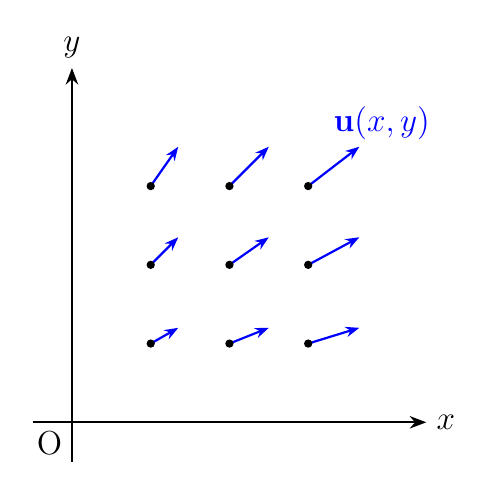
\begin{tikzpicture}[every node/.style={font=\large}]
  % Axes
  \draw[-{Stealth[length=6pt]}, thick] (-0.5,0) -- (4.5,0) node[right] {$x$};
  \draw[-{Stealth[length=6pt]}, thick] (0,-0.5) -- (0,4.5) node[above] {$y$};
  \node[below left] at (0,0) {O};

  % Vector field arrows at grid points
  \foreach \x/\y/\dx/\dy in {
    1/1/0.35/0.2,
    2/1/0.5/0.2,
    3/1/0.65/0.2,
    1/2/0.35/0.35,
    2/2/0.5/0.35,
    3/2/0.65/0.35,
    1/3/0.35/0.5,
    2/3/0.5/0.5,
    3/3/0.65/0.5
  } {
    \draw[-{Stealth[length=5pt]}, thick, blue] (\x,\y) -- +(\dx,\dy);
    \fill (\x,\y) circle (1.5pt);
  }

  % Label
  \node[blue, right] at (3.2,3.8) {$\mathbf{u}(x,y)$};
\end{tikzpicture}
\end{document}
